% AAMAS 2027 anonymous research-track revision, submission 1979.
% The official aamas.cls and bibliography style are copied unchanged.
% Preserve the format of native vector diagram exports; no layout override.
\ifdefined\pdfminorversion\pdfminorversion=7\relax\fi
\documentclass[sigconf,anonymous]{aamas}
% Compatibility guard for the unchanged class's incomplete default metadata.
\makeatletter
\def\AAMAS@orphanfi{\fi}
\def\AAMAS@repairconference{%
  \acmConference@editors
  \global\let\acmConference@editors\@empty}
\ifx\acmConference@editors\AAMAS@orphanfi
  \expandafter\AAMAS@repairconference
\fi
\makeatother
\usepackage{balance}
\usepackage{amsmath}
\usepackage{algorithm}
\usepackage{algpseudocode}

% Official AAMAS 2027 copyright block (unchanged from the supplied template).
\makeatletter
\gdef\@copyrightpermission{
  \begin{minipage}{0.2\columnwidth}
   \href{https://creativecommons.org/licenses/by/4.0/}{
\includegraphics[width=0.90\textwidth]{by}}
  \end{minipage}\hfill
  \begin{minipage}{0.8\columnwidth}
   \href{https://creativecommons.org/licenses/by/4.0/}{This work is licensed under a Creative Commons Attribution International 4.0 License.}
  \end{minipage}
  \vspace{5pt}
}
\makeatother
\setcopyright{ifaamas}
\acmConference[AAMAS 2027]{Proc.\@ of the 26th International Conference
on Autonomous Agents and Multiagent Systems (AAMAS 2027)}{3--7 May 2027}{Hanoi, Vietnam}{M.~Baldoni, F.~Fang, W.~Yeoh, N.~Yorke-Smith (eds.)}
\copyrightyear{2027}
\acmYear{2027}
\acmDOI{}
\acmISBN{}
\acmSubmissionID{1979}
\submissionType{Research Paper Track}
\title{Learning Joint Recovery of Multi-Agent Graph Optimization for Satellite--Ground Scheduling}

% Author names are retained separately in submission_metadata.json.
% Affiliations and emails are not inferred. The submission remains anonymous.
\begin{abstract}
In multi-agent satellite--ground scheduling, a coordinated adjustment is valuable
only when its immediate change and recovered contacts form a compatible
schedule. Summing individual replacement values can overestimate improvement,
while solving every candidate can exhaust the decision budget. We formulate
learning the additional joint recovery beyond a shared, executed greedy
response. An action-conditioned graph encoder represents eligible contacts,
conflict factors and actual warm membership. A request-aware head combines
fractional capacity features with warm and budget context to predict finite
recovery between a feasible lower value and a clique-partition upper bound;
the known immediate gain is added separately. Training compares alternative
requests executed from cloned states, using signed values, improvement rankings
and feasible membership supervision. At deployment, predictions prioritize
finite executor calls while an independent kernel checks complete schedules
and preserves the incumbent. Quality measures feasible improvement actually
received before the total deadline, charging preparation, inference, execution
and final checks.
Controlled experiments identify substantial conditional recovery opportunity,
but distinguish it from realized policy quality: longer allowances permit
additional recovery, while inexpensive summary and greedy controls remain
competitive and strict short deadlines expose the cost of allocation.
Profiles of seven published native configurations and three released neural
recipes on 40 public graphs provide a complementary solver comparison.
The results clarify when joint recovery is an informative learning target
and why structural prediction alone does not guarantee better timed schedules.

\end{abstract}
\ccsdesc[500]{Computing methodologies~Multi-agent systems}
\ccsdesc[500]{Mathematics of computing~Combinatorial optimization}
\ccsdesc[300]{Computing methodologies~Neural networks}
\keywords{Multi-agent coordination, graph learning, maximum-weight independent set, satellite scheduling, learned local search}

\newcommand{\score}{f_{\theta}}
\newcommand{\weight}[1]{w(#1)}
\newcommand{\kernel}{\mathcal{K}_{B}}
\newcommand{\actions}{\mathcal{A}}
\newcommand{\response}{\mathcal{H}}
\newcommand{\method}{JointRecovery}

\begin{document}
\maketitle
\section{Introduction}
\label{sec:introduction}

Satellite--ground scheduling allocates contact opportunities that compete
for satellite and ground-station resources. When contacts belong to
different agents, replacing one agent's commitments can displace another's
assignments and change the alternatives available to both. This connects
schedule improvement to the resource-coupled coordination studied in
multi-agent constellation scheduling~\cite{picard2022satellite} and
constraint optimization~\cite{fioretto2018}. We study a centralized
coordinator operating on an owner-partitioned conflict graph: contacts are
weighted vertices, incompatible contacts are adjacent, and a feasible
schedule is an independent set. Agent partitions identify which owners an
adjustment affects; resource conflicts determine its feasibility.

The value of a coordinated adjustment depends on what can be recovered
after its immediate insertions and withdrawals. Individually attractive
alternatives cannot generally be added: one reward-$10$ contact may exclude
two compatible reward-$6$ contacts, whose joint value is $12$. An action
with a smaller immediate gain can therefore yield a better completed
schedule when its replacements are mutually compatible. Explicitly repairing
every action evaluates executable joint outcomes, but spends the
decision allowance on alternatives that may never be executed. The useful
prediction target is consequently the improvement obtainable by a specified
finite repair procedure, conditioned on its recovery scope and actual warm
start, rather than an unbudgeted optimum or a sum of individual values.
Figure~\ref{fig:problem-joint-recovery-v4} illustrates how incompatible
replacements can reverse the preferred adjustment.

\begin{figure}[t]
  \centering
  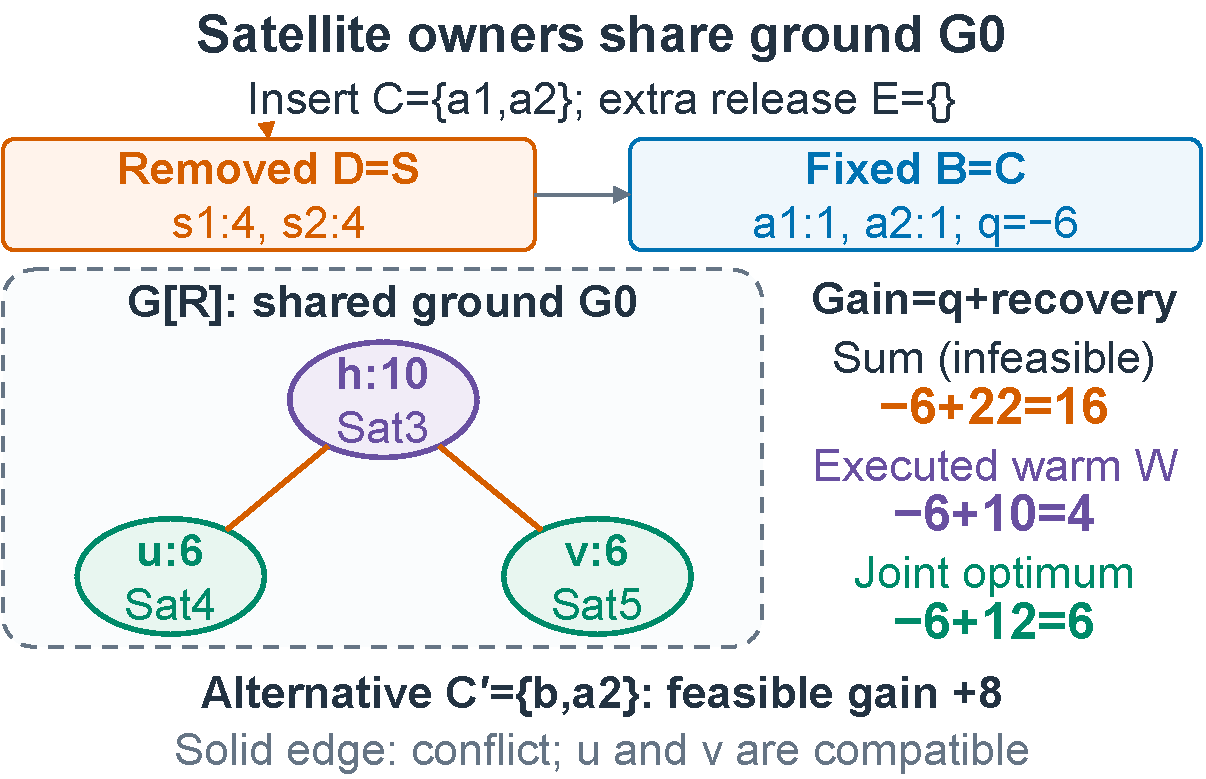
\includegraphics[width=\columnwidth]{v4_figures/residual_schematics/problem_joint_recovery.pdf}
  \caption{Constructed contact example with satellite ownership. Inserting $C$ displaces $D=S$ and fixes $B$, giving $q=-6$. Separate owner recoveries sum to $22$ but conflict on ground G0. All three shared greedy rules return $W=\{h\}$, worth $10$; the compatible joint pair $\{u,v\}$ is worth $12$. Independent addition incorrectly prefers $C$ to the feasible alternative $C'$ with gain $8$; joint recovery reverses this choice. This is a mathematical illustration, not an experimental result.}
  \label{fig:problem-joint-recovery-v4}
\end{figure}


Learning already guides decisions inside combinatorial solvers and selects
subproblems for classical repair~\cite{gasse2019branching,li2021delegate}.
Our focus is the joint recovery value of coordinated adjustments under a
complete decision-time budget. Each action fixes a base schedule and induces
an eligible recovery graph. We represent the remaining alternatives through
their conflicts, resource factors, weights, and observed warm-start
membership. The representation is action-conditioned through this induced
scope; it does not require learning the known immediate gain. Crucially,
every policy first executes a common greedy recovery. The learner estimates
additional joint recoverability between this actual feasible lower value and
a structural upper bound. Sparse fractional occupancies expose competition
among replacements inside that interval; the execution kernel supplies
actual memberships and enforces feasibility.

Finite recovery also depends on how much work the executor receives and
what it has already recovered. We separate these quantities in a factorized
predictor: one structural encoding is shared across requests with the same
recovery graph, factors, and actual warm start, while small heads condition
on the native workpoint and remaining allowance. The immediate gain enters
as an exact final offset. The controller uses these predictions to allocate
paid finite solver calls and retains only validated improvements. Changing
the observed warm start changes the structural input; predictions never
supply an unexecuted recovery as their own warm start.

The paper develops three mechanisms for testing this approach:
\begin{itemize}
  \item A warm-anchored joint recovery predictor that separates a shared,
  already executed greedy value from possible additional recovery, using
  conflicts, resource factors and actual warm membership.
  \item An execution-aligned supervision protocol that compares actual
  finite outcomes from the same state, retaining signed gains, returned
  memberships, failures, and late outcomes.
  \item A factorized finite-call allocator and complete-cost comparison
  protocol covering the declared classical portfolio and matched structural,
  supervision, and warm-start controls.
\end{itemize}

The primary criterion is the objective of the feasible schedule finally
validated and returned within a common total allowance $D$. Proposals,
representation preparation, inference, repair, and final validation are all
charged; a late return receives the original incumbent for this criterion.
We distinguish an improvement available internally before $D$ from timely
return. The completed evaluation covers controlled
coupling graphs and interval-resource scheduling graphs, together with
separate profiles of published solvers on original public graph tasks.
These public profiles establish solver behavior and execution costs;
they do not establish transfer of our learned policy. The central question is whether joint recovery
structure provides useful allocation information beyond strong inexpensive
priorities when every policy pays the same complete decision cost.
The evidence separates the usefulness of the recovery target from the
performance of this particular allocator: finite recovery remains available,
but preparation and caller latency can dominate small decision budgets.

\section{Related Work}
\label{sec:related}

\paragraph{Multi-agent coordination and scheduling.}
Satellite constellation scheduling already combines auctions and distributed
constraint optimization to coordinate users holding exclusive orbit
portions~\cite{picard2022satellite}. Consensus-based allocation also handles
multi-mode composite requests whose constituent tasks require several slot
owners to revise their schedules~\cite{picard2023composite}. These models
establish that the benefit of an allocation can depend on coordinated
schedule changes. Coalition action selection further learns simultaneous
combinatorial allocations in online resource
allocation~\cite{gebrekidan2024coalition}. Our owner-partitioned contact graph
focuses on the recovery induced by a proposed adjustment: displaced and
newly available contacts must be compatible with both the fixed commitments
and one another. Ownership identifies the participating agents; our central
execution procedure does not establish a distributed communication protocol
or the privacy guarantees of the satellite allocation methods.

\paragraph{MWIS algorithms.}
Weighted branch-and-reduce combines exact data reductions with branching
for MWIS~\cite{lamm2019exact}. Struction extends this approach with
transformations that can enlarge a graph to expose further
reductions~\cite{gellner2021struction}. The memetic algorithm
$m^2$wis combines population search with recursive vertex selection and
data reduction~\cite{grossmann2024mwis}, while CHILS supplies concurrent
iterated local search and can also exploit parallel
execution~\cite{grossmann2025chils}. These are substantial weighted search
methods and relevant whole-graph baselines, as well as potential recovery
executors. Our learned controller allocates finite recovery calls; it does
not certify their optimality. Whole-graph solving and selection among
action-induced recovery requests have different inputs and initialization
contracts. We therefore distinguish published-solver comparisons from
comparisons in which policies share the incumbent, action pool, scopes,
executor, and available workpoints.

\paragraph{Learning independent sets and improvement.}
DIFUSCO generates graph solutions by denoising binary selection
vectors~\cite{sun2023difusco}; COExpander uses global predictions to guide
adaptive expansion of determined partial
solutions~\cite{ma2025coexpander}. Their MIS evaluations concern constructing
independent sets, and our comparisons retain their supported unit-weight
task. Learning local revision is also established: neural rewriting
learns successive changes to an existing
solution~\cite{chen2019}. Learning to Delegate is particularly close: it
predicts a blackbox subsolver's resulting cost, obtains training labels by
executing candidate subproblems from a current solution, and retains the
current subsolution when a replacement fails to
improve it~\cite{li2021delegate}. Thus, neither learned repair selection nor
supervision from solver outcomes is new here.

\paragraph{Execution-conditioned value and computation.}
Data-driven heuristic scheduling already uses observed call durations and
success to determine which primal heuristics to run and for how
long~\cite{chmiela2021schedule}. Decision-focused learning likewise aligns
predictions with downstream decisions, including through ranking
losses~\cite{mandi2022rank}. Classical clique inequalities provide established
constraints on compatible vertex selections~\cite{chvatal1975polytopes}.
Our narrower target is the jointly executable recovery value conditional
on an adjustment, recovery scope, finite solver workpoint, and actual warm
start. Alternatives share the same incumbent snapshot, and labels record
the feasible outcomes actually produced by the execution procedure.
The model represents conflicts within the recovery set rather than summing
isolated replacement values. Its benefit must be assessed against
nonlearned allocation using the same execution options, charging preparation, inference,
execution, validation, and return. The primary quantity is the feasible
improvement received by the caller before the total deadline; internally
available or late solutions are separate measurements. This formulation
poses an empirical question about decision quality per complete online
budget, without presuming an advantage over existing search.

\section{Problem and Executable Joint Recovery}
\label{sec:problem}

An owner-partitioned conflict graph is $G=(V,\mathcal E,w,\alpha)$,
where $w_v\geq0$ and $\alpha:V\to\{1,\ldots,m\}$ assigns vertices to
agents. Writing $w(U)=\sum_{v\in U}w_v$, a feasible schedule is an
independent set; maximum-weight independent set (MWIS) maximizes $w(S)$
over such sets.
In satellite--ground scheduling, vertices represent contacts, satellite
agents own their contacts, and shared satellite or ground resources induce
conflicts. Ownership adds no one-contact-per-agent constraint or communication
protocol. The public-graph partition $\alpha(v)=1+(v\bmod8)$ is artificial;
it does not encode satellite or ground-station ownership.

Given an independent incumbent $S$, an action $a=(C_a,E_a)$ commits an
independent $C_a\subseteq V\setminus S$ and optionally releases
$E_a\subseteq S$. With $N(U)=\bigcup_{v\in U}N(v)$, define
\begin{align}
 D_a&=(N(C_a)\cap S)\cup E_a,\qquad
 B_a=(S\setminus D_a)\cup C_a,\nonumber\\
 q_a&=w(C_a)-w(D_a).\label{eq:v4-action-base}
\end{align}
The action pool uses eleven target cells:
$|C_a|\in\{0,2,4,8\}$ and release targets $\{0,16,64\}$, excluding
the empty action. Actual releases can be fewer; unavailable and duplicate
actions do not create additional queries. Admissible adjustments span at
least two owner partitions. Pure release actions have $C_a=\emptyset$.

Recovery candidates must be compatible with the entire fixed base:
\begin{equation}
 U_a=(D_a\cup N(D_a))\setminus(B_a\cup N(B_a)),\quad
 R_{a,r}=\operatorname{prefix}_r(U_a).
 \label{eq:v4-recovery-scope}
\end{equation}
The ordering places restorable incumbent vertices first, then other vertices
by decreasing reward and identifier. We fix $r=256$ for both the learned
method and its matched controls. Changing $E_a$ changes the action and base,
rather than the amount of information supplied to one policy. Equal actual
prefixes share one request identity.

\begin{proposition}[Feasible recovery and exact gain]
\label{prop:v4-recovery-decomposition}
For any independent $T\subseteq R_{a,r}$, $B_a\cup T$ is feasible and
\begin{equation}
 w(B_a\cup T)-w(S)=q_a+w(T).
 \label{eq:v4-realized-decomposition}
\end{equation}
In particular, $S\cap R_{a,r}$ is a feasible known recovery.
\end{proposition}
\begin{proof}
Removing $N(C_a)\cap S$ makes $B_a$ independent. Every vertex in $R_{a,r}$
is outside and nonadjacent to $B_a$, so independent $T$ completes it
feasibly. Disjointness gives the weight identity. The incumbent intersection
inherits independence from $S$.
\end{proof}

A request specifies $(a,256,\kappa)$, with finite executor workpoint $\kappa$
in its declared native unit. Every policy first executes the same greedy
portfolio on the recovery graph and compares its actual memberships with
$S\cap R_{a,256}$. Its best feasible membership initializes the warm start
$W$. Earlier, timely same-action recoveries can improve $W$. The executor returns an actual recovery $T$
or a failure; full membership validation and rescoring determine its signed
gain in Eq.~\eqref{eq:v4-realized-decomposition}. Neither finite execution
nor a fractional occupancy estimate is an exact recovery oracle.

For total decision allowance $D$, a policy pays for proposals, scope and
priority preparation, inference, execution, and final validation within the
same decision. Let $S_\pi^{\rm ret}(D)$ be its feasible, nondecreasing
schedule actually received by the caller strictly before $t_0+D$, and set
$S_\pi^{\rm ret}(D)=S$ otherwise. The primary objective is
$g_\pi(D)=w(S_\pi^{\rm ret}(D))-w(S)$.
Internal availability before $D$ is a separate quantity. The target is
executable improvement under a complete return deadline, rather than a sum
of individual replacements or the best recovery found after the deadline.

\begin{figure*}[t]
  \centering
  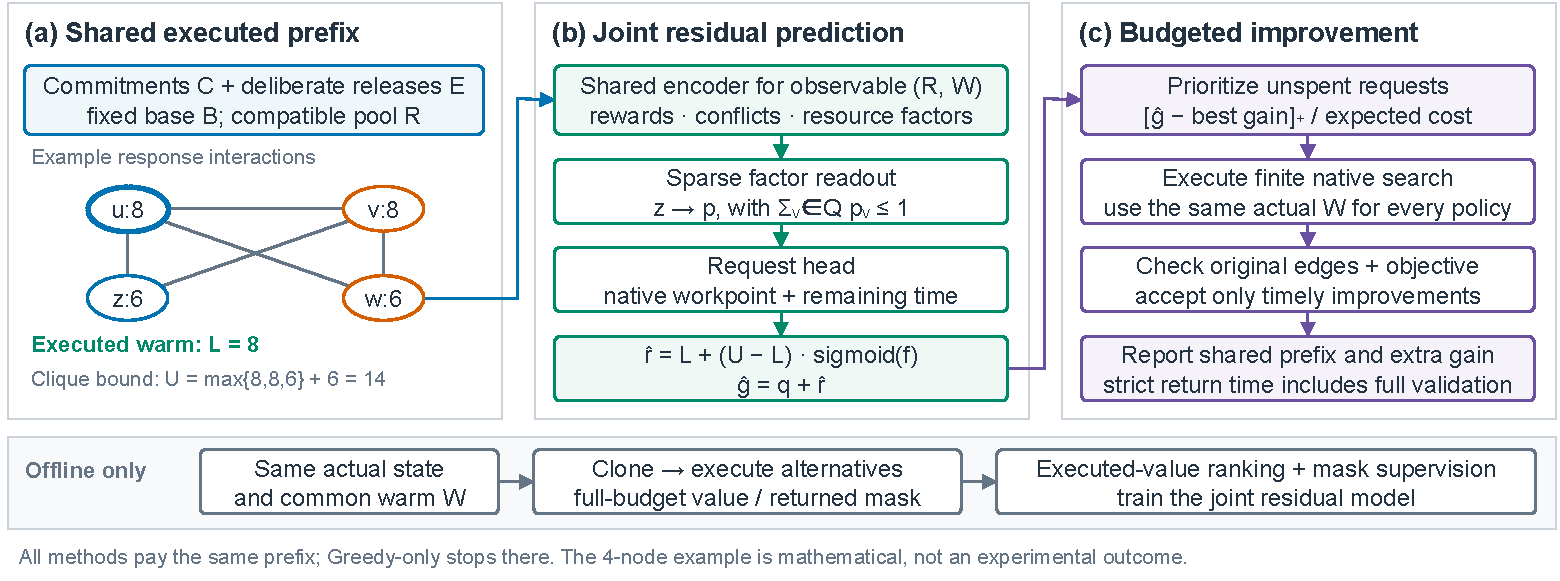
\includegraphics[width=\textwidth]{v4_figures/residual_schematics/method_joint_residual.pdf}
  \caption{Learning additional joint recovery after a common executed greedy
  response. (a) Each commitment/release action determines a fixed base and
  compatible recovery graph. The mathematical four-vertex example has greedy
  value $L=8$, joint optimum $12$, and clique-partition bound $U=14$.
  (b) A shared structural encoder, request-conditioned fractional occupancies,
  and bounded residual head estimate further finite recovery; the known
  immediate gain enters as an exact offset. (c) Predictions prioritize calls
  using the same actual warm membership, while the execution kernel admits
  only validated improvements. Training compares executed alternatives from
  the same snapshot. The example is illustrative, not an empirical result.}
  \label{fig:method-residual}
\end{figure*}

\section{Learning Additional Finite Joint Recovery}
\label{sec:method-residual}

The learned quantity is additional joint recovery beyond a shared, executed
greedy response. Learned subproblem delegation and heuristic scheduling
already use solver outcomes and computation allowances~\cite{li2021delegate,chmiela2021schedule}.
Our formulation combines coordinated recovery structure, an actual feasible
warm anchor, and finite-execution supervision to prioritize further calls.
It does not introduce graph message passing, clique inequalities, or
budget allocation themselves.

\subsection{Shared Executed Recovery}
For each available commitment/release action from Section~\ref{sec:problem},
we fix $R=R_{a,256}$. Proposals depend on observable weights, conflicts,
ownership and a fixed exploratory seed, rather than recovery outcomes.
Commitments use a shared pool of high immediate-gain and exploratory
vertices; releases follow a seeded incumbent-boundary traversal.
Ownership restricts coordinated proposals to multiple partitions; it is
not an additional feasibility constraint. Changing commitments or releases
changes the base $B_a$ and recovery eligibility, rather than simply enlarging
a neighborhood.

Every policy executes three greedy sweeps on $G[R]$, ordering vertices by
$w_i/(1+d_i)^e$ for $e\in\{0,\frac12,1\}$, with deterministic weight and
identifier ties. Each sweep inserts a vertex only when compatible with its
current selection. Comparing their actual feasible memberships with
$S\cap R$ gives the best known warm recovery $W$. Full validation of
$B_a\cup W$ precedes incumbent admission. Construction, sweeps, and
validation consume the common decision allowance. A greedy-only policy
returns after this prefix; its improvement is shared preparation, not a
learning gain. Subsequent calls use $W$, updated only by better, timely,
validated same-action responses.

\subsection{Action-Conditioned Structural Representation}
The encoder sees the induced recovery conflict graph and genuine clique
factors $\mathcal F_R$. Factors comprise supplied resource cliques restricted
to $R$, greedily grown conflict cliques, and uncovered edges as two-vertex
cliques. No maximal-clique enumeration is required. Fixed commitments and
displacements determine eligibility before encoding; they are not separate
message-passing nodes. Agent identifiers are not neural inputs, and the
encoder does not learn an inter-agent communication protocol.

With scale $s_G=\max(1,|V|^{-1}\sum_v w_v)$, vertex features contain
normalized weight, logarithmic and normalized conflict degree, actual warm
membership, and incident-factor count and size statistics. A width-32,
two-layer encoder applies
\begin{equation}
 \begin{aligned}
 h_i^{\ell+1}=\operatorname{ReLU}\!\Bigl(&A_\ell h_i^\ell+
 B_\ell\operatorname{mean}_{j\in N_R(i)}h_j^\ell\\
 &+D_\ell\operatorname{mean}_{F\ni i}\operatorname{mean}_{j\in F}h_j^\ell
 \Bigr).
 \end{aligned}
 \label{eq:residual-encoder}
\end{equation}
Empty means are zero. Mean and weight-normalized mean pooling summarize
the recovery set. The request head also receives native workpoint type and
amount, remaining time, actual warm reward and fraction, and scalar
weight, density, factor and classical-bound summaries. The current best
gain is used by the allocation rule below, rather than the encoder.

Encoding is independent of the known immediate gain $q_a$ and request
allowance. Inference reuses representations only for identical ordered
recovery vertices, factors, warm membership and scale within the same graph
and model version. Warm changes require a new encoding. Cache preparation,
lookups, packing and device transfers remain paid online operations;
training uses no detached embedding cache.

\subsection{A Warm-Anchored Residual Value}
Let $L=w(W)$. A deterministic traversal of genuine cliques partitions $R$
into disjoint residual clique blocks and leftover singletons,
$\mathcal P_R$. Consequently,
\begin{equation}
 U=\sum_{Q\in\mathcal P_R}\max_{i\in Q}w_i
 \quad\text{satisfies}\quad L\leq\operatorname{MWIS}(G[R])\leq U.
 \label{eq:residual-upper}
\end{equation}
This classical upper bound need not be tight~\cite{chvatal1975polytopes}.

Request-conditioned logits $\ell_i$ produce sparse occupancies
\begin{equation}
 p_i=\sigma(\ell_i),\qquad
 z_i=\frac{p_i}{\max\{1,\max_{F\ni i}\sum_{j\in F}p_j\}}.
 \label{eq:residual-occupancy}
\end{equation}
All incident loads are computed simultaneously. Hence
$\sum_{i\in F}z_i\leq1$ for each factor, including covered conflict edges.
These are fractional compatibility features, not executable memberships.
Their weighted sum, normalized by $U$ with a numerical zero safeguard,
joins the pooled encodings and request context in a width-32 residual head:
\begin{equation}
 \widehat r=L+(U-L)\sigma(f_\theta),\qquad
 \widehat t=q_a+\widehat r.
 \label{eq:residual-value}
\end{equation}
The head's final bias is initialized to $-4$. Computation uses normalized
weights and restores native units at readout. The occupancy sum is not
$\widehat r$: the latter is a bounded scalar estimate of finite recovery.
For example, $L=8$, $U=14$ and joint optimum $12$ illustrate distinct
warm, bound and joint values in the mathematical schematic; they are not
experimental observations. Neither bound nor prediction certifies the
executor's finite outcome.

\subsection{Execution-Aligned Supervision}
Each graph supplies two equally weighted snapshots: after the paid common
prefix, and after at most one actually startable, fixed-order history call
using the same remaining decision budget. Every alternative clones the
same current best, warm memberships, spent requests and remaining time.
Executing one alternative never warms another. The procedure's returned $T_j$,
including its retained actual warm start when no new native output is available,
is fully checked against the original graph and fixed base. Valid responses
provide signed target $t_j=(q_{a_j}+w(T_j))/s_G$ and binary membership
$m_{ji}=\mathbf1[i\in T_j]$, even when late. The admitted target $y_j$ is
$[t_j]_+$ only if validation finishes strictly before the snapshot deadline;
otherwise it is zero. Failed calls retain zero-admission ranking targets
without invented raw or mask targets. Unstartable alternatives remain in
coverage but are excluded from model batches.
Executed targets enter the loss, never the encoder or inference cache.

For snapshot $s$, let $\widetilde t_j=\widehat t_j/s_G$,
$\mathcal V_s$ be valid returned responses,
$b_s$ its normalized best gain, and
$\delta_j=[y_j-b_s]_+$. Define
\begin{align}
 \mathcal L_s={}&\operatorname{mean}_{j\in\mathcal V_s}
    \operatorname{SmoothL1}(\widetilde t_j,t_j)\nonumber\\
 &+\operatorname{mean}_{\delta_j>\delta_k}
    \operatorname{softplus}\!\left(-\frac{\widetilde t_j-\widetilde t_k}{0.2}\right)
    +0.05\mathcal L_s^{\rm mask}.
 \label{eq:residual-loss}
\end{align}
Mask loss averages nodewise logit BCE within each valid nonempty response,
then across responses. Empty means are zero. Signed prediction differences
remain unclamped. For domain $d$ with $n_d$ graphs, the objective is
$\sum_G(\mathcal L_{G,0}+\mathcal L_{G,1})/(4n_{d(G)})$.
This gives equal domain mass and half weight to each snapshot, without
reweighting empty states. Checkpoint selection uses offline conditional
allocation regret, a proxy distinct from complete online return quality.

\subsection{Finite Allocation and Feasible Return}
For current best gain $g^*$ and shared expected call cost $c_j$, requests
are ordered by $[\widehat t_j-g^*]_+/c_j$, then $[\widehat t_j]_+/c_j$
and fixed request order. This point-marginal heuristic is not
$\mathbb E[(G_j-g^*)_+]$ for random admitted gain $G_j$. Only unspent requests whose native allowance and
expected cost fit the remaining time can start, with at most eight calls.
Every started call, including failure or overrun, is spent. The executor
receives the actual $W$; its finite response is independently materialized,
validated and rescored. Integer objectives use native exact sums. A timely
strict improvement updates the incumbent; other responses preserve it.
Final validation, synchronization and actual caller receipt must precede
the total deadline, otherwise the primary return is the original $S$.

The matched controls FreeOccupancy, NoAux, NoWarm and CheapSummary
omit occupancy contraction, mask BCE, warm membership identity, or graph
encoding, respectively. All retain the same executed $W$, scalar $L$,
upper bound and execution options; removing warm identity keeps native warm
starts unchanged. The learned point estimate only chooses execution order.
Feasibility and nondecrease come from the kernel, and additional benefit
must be measured above the common greedy prefix.

\section{Experimental Design}
\label{sec:experiments}

The protocol asks whether predicting additional joint recovery improves
complete-decision quality beyond an executed greedy response; whether
compatibility structure, occupancy supervision and warm information explain
any improvement; and how published solvers behave on public graph
optimization tasks. Published whole-graph
solvers and priorities within a shared recovery kernel answer complementary
questions. Performance tables pair each published method with its citation
and execution cost; implementation configurations are provided separately.

\paragraph{Controlled tasks and splits.}
Recovery menus cross 64/256 alternatives per menu, eight menus, three
topologies (Erd\H{o}s--R\'enyi, components, bipartite), densities
$0.08/0.20/0.45$, and cross-menu coupling $0.04$. Resource graphs cross
48/96 visibility passes with two/four/eight ground stations, eight
satellites and six alternatives per pass. Their conflicts represent
satellite and ground occupation. These 18 menu and six resource cells
define 72 training and 24 validation graphs, with graph-seed splits preceding
action/state extraction. All policy results use the complete 24-graph
development validation split. Previously inspected public inputs remain
exposed benchmark data.

\paragraph{Published whole-graph comparisons.}
The completed public comparison retains all 40 original unit-weight graphs:
16 DIMACS clique complements~\cite{johnson1996dimacs}, 18 SATLIB UF and six
CBS clause-conflict graphs~\cite{hoos2000satlib}, each with three common
initial schedules. The seven native configurations are CHILS-p1 and
CHILS-p16-c16~\cite{grossmann2025chils}, the two
$m^2$wis variants~\cite{grossmann2024mwis}, both Struction
configurations~\cite{gellner2021struction}, and
WeightedBR~\cite{lamm2019exact}. Their $0.5/2$\,s soft search workpoints
give 1,680 runs. The 16-thread CHILS configuration is reported separately
from single-thread configurations. Three released neural recipes add 360
runs: DIFUSCO-SAT with 50 steps and one/four
samples~\cite{sun2023difusco}, and COExpander-SAT-CM with one
sample (CM $1\times1$)~\cite{ma2025coexpander}. Raw and accepted cardinalities
are reported separately. Released-model
training overlap is unresolved, so this benchmark is a transfer comparison.

\paragraph{Numerical and application scope.}
The public benchmark uses the original unit rewards and conflict edges,
so released unit-MIS models are evaluated within their mathematical domain.
The controlled resource family retains satellite and station interval
conflicts and positive rewards. We do not extrapolate released unit-MIS
models to weighted contact scheduling. Large original contact sources and
weighted route benchmarks require separate numerical-domain and policy
transfer experiments; they are not part of the completed policy comparison.

\paragraph{Matched recovery controls.}
Every policy uses the same eleven commitment/release cells
$|C|\in\{0,2,4,8\}$, $|E|\in\{0,16,64\}$, excluding the no-op, and
fixed replacement cap of 256. The common paid prefix executes all three
weight/degree greedy sweeps and compares their feasible memberships with
$S\cap R$, yielding $W$. AnytimeGreedyPortfolio (greedy-only) returns this prefix;
Lower reuses it without repeating sweeps. Immediate, Upper, P1, Lower and
RoundRobin prioritize the same CHILS-p1 requests: one thread, seed 17,
10/50/200\,ms workpoints and at most eight calls. Upper uses a
clique-partition bound; P1 uses clique-load discounts. Unavailable cells remain
in coverage. All methods share
feasibility checks and incumbent preservation.

\paragraph{Learned controls and selection.}
Capacity and the FreeOccupancy, NoAux, NoWarm and CheapSummary controls
retain the same $W$, lower and upper bounds, and execution options.
NoWarm masks warm indicators and warm fraction while retaining scalar
$L=w(W)$. The label design clones two actual execution snapshots under
the revised warm semantics. Before fitting, the protocol requires measuring
native extra above the shared prefix across the full pool. Graph encoders
use width 32 and two layers; training fixes Adam $10^{-3}$,
four-graph batches and 40 epochs. All seeds 17/29/43 contribute;
each fit selects its first minimum validation
conditional regret. The strongest of all six classical controls at
$D=0.556$\,s is selected using the complete validation grid.

\paragraph{Quality, cost and statistics.}
Measured runs use Linux, an RTX 4080 and PyTorch 1.11/CUDA 11.3;
native solvers use one thread except the separately marked CHILS-p16-c16.
The total deadlines are 0.139, 0.556 and 2.221\,s. We normalize the
timely gain $g_\pi(D)$ by $\max\{1,w(S)\}$; a late return retains $S$.
Timing includes
proposals, scopes, features, bounds, inference, transfers, native execution,
validation/rescoring, synchronization and caller return. Common-prefix gain and
additional returned gain are reported separately from source availability.
Resident graph/model setup is separate; each decision starts with empty
caches. Native cold wall time includes export, startup, parsing and validation;
neural resident request time and once-only setup remain separate from
native soft stops and controller deadlines. They do not establish a
matched-budget speedup.

Fits and initial seeds are averaged within each graph before aggregation.
Controlled domains receive equal mass; public DIMACS/UF/CBS means receive
equal family weight. Failures, late returns and zero-opportunity graphs keep
their original mass; N/A remains distinct from executable failure.
Queries and repeated fits are not independent observations. Paired graph
bootstrap intervals describe development uncertainty, resampling graphs
within each domain and retaining equal domain weight. They do not constitute
an independent confirmation test.

\section{Results}
\label{sec:results-residual}

\paragraph{Complete-decision quality at the primary budget.}
Table~\ref{tab:main-runtime-ablation} compares \method{} (Capacity), all six
classical priorities, and four matched learned controls. All 15 fits and
24 validation graphs contribute to the 1,512 complete decisions across
three deadlines. Fitting seeds are averaged within each graph before
assigning equal mass to the menu and resource domains. The gain is the
strictly returned improvement relative to the original incumbent, not the
best solution internally available before caller return.

Figure~\ref{fig:online-budget-v4} separates complete return quality,
additional recovery, and caller deadline misses. At the primary
$D=0.556$\,s, Capacity returns 57.542\% gain, while the greedy-only
policy returns the shared prefix's 234.266\% gain in 0.035\,s.
Capacity's 83.333\% late-return rate removes otherwise materialized
improvements from the strict objective. The primary comparison therefore
does not establish a learned-policy advantage; Section~\ref{sec:discussion-residual}
discusses the implications for finite allocation. Longer allowances expose
the additional recovery that a short complete deadline cannot retain.

\begin{table*}[t]
\centering
\caption{\textbf{Complete-decision comparison on all 24 validation graphs.}
Gain: timely improvement over the original incumbent (\%, higher is better).
Late: caller deadline-miss fraction. Time: actual caller latency (s), including
late returns. Aggregation is graph-first and domain-balanced; bold marks the
highest mean at each deadline, without a significance claim.}
\label{tab:main-runtime-ablation}
\footnotesize
\setlength{\tabcolsep}{4pt}
\begin{tabular}{@{}lrrrrrrrrr@{}}
\toprule
& \multicolumn{3}{c}{$D=0.139$\,s} & \multicolumn{3}{c}{$D=0.556$\,s (primary)} & \multicolumn{3}{c}{$D=2.221$\,s} \\
\cmidrule(lr){2-4}\cmidrule(lr){5-7}\cmidrule(lr){8-10}
Method & Gain $\uparrow$ & Late $\downarrow$ & Time $\downarrow$ & Gain $\uparrow$ & Late $\downarrow$ & Time $\downarrow$ & Gain $\uparrow$ & Late $\downarrow$ & Time $\downarrow$ \\
\midrule
\textbf{\method{} (Capacity)} & 74.887 & 0.861 & 0.240 & 57.542 & 0.833 & 0.642 & 236.334 & 0.000 & 1.725 \\
\midrule
AnytimeGreedyPortfolio & \textbf{234.266} & 0.000 & 0.035 & \textbf{234.266} & 0.000 & 0.035 & 234.266 & 0.000 & 0.035 \\
Immediate & 21.107 & 0.944 & 0.232 & 21.107 & 0.944 & 0.634 & 234.624 & 0.000 & 1.429 \\
Upper & 108.040 & 0.778 & 0.218 & 43.078 & 0.889 & 0.642 & 234.266 & 0.000 & 1.606 \\
PairPriority (P1) & 78.310 & 0.861 & 0.230 & 56.909 & 0.889 & 0.648 & 236.218 & 0.000 & 1.474 \\
Lower & 21.107 & 0.944 & 0.234 & 0.000 & 1.000 & 0.651 & 234.393 & 0.000 & 1.602 \\
RoundRobin & 21.107 & 0.944 & 0.231 & 13.348 & 0.972 & 0.636 & 234.266 & 0.000 & 1.480 \\
\midrule
FreeOccupancy & 76.759 & 0.861 & 0.240 & 43.099 & 0.889 & 0.650 & 237.007 & 0.000 & 1.696 \\
NoAux & 80.406 & 0.852 & 0.240 & 51.799 & 0.843 & 0.642 & 236.916 & 0.000 & 1.726 \\
NoWarm & 71.939 & 0.870 & 0.238 & 69.318 & 0.833 & 0.642 & 236.891 & 0.000 & 1.721 \\
CheapSummary & 73.834 & 0.861 & 0.230 & 94.665 & 0.806 & 0.645 & \textbf{238.355} & 0.000 & 1.674 \\
\bottomrule
\end{tabular}
\par\smallskip
\begin{minipage}{\textwidth}
\footnotesize
All methods share the executed greedy prefix; every native request uses
the CHILS-p1 recovery kernel~\cite{grossmann2025chils}. Upper uses the classical clique
bound~\cite{chvatal1975polytopes}. These are matched allocation controls,
not separate published whole-graph solvers. All graph and fit slots retain
their prescribed weights; a late final return receives zero strict gain.
Once-only resident graph/model setup is excluded from decision time.
\end{minipage}
\end{table*}

\begin{figure*}[t]
\centering
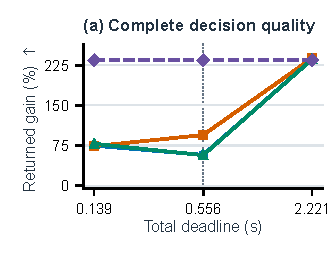
\includegraphics[width=0.326\textwidth]{v4_figures/residual_results/online_quality.pdf}\hfill
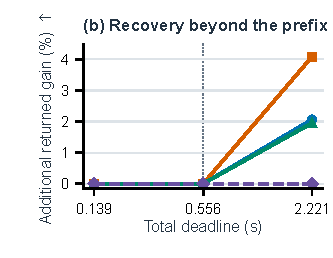
\includegraphics[width=0.326\textwidth]{v4_figures/residual_results/online_extra.pdf}\hfill
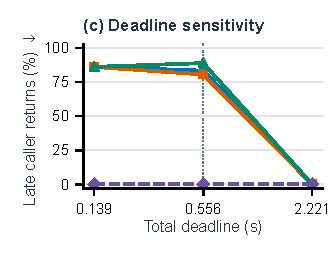
\includegraphics[width=0.326\textwidth]{v4_figures/residual_results/online_lateness.pdf}\\

\includegraphics[width=0.94\textwidth]{v4_figures/residual_results/online_legend.pdf}
\caption{\textbf{Joint recovery under complete decision budgets.}
All 1,512 runs use graph-first, equal-domain aggregation.
(a) Validated gain actually received before the deadline.
(b) Additional gain beyond the paid common prefix.
(c) Caller deadline misses, retaining the original schedule in (a).
Dotted lines mark the primary deadline. Longer budgets admit extra recovery;
CheapSummary remains competitive with the structural predictor.}
\label{fig:online-budget-v4}
\end{figure*}


\paragraph{Longer budgets and matched components.}
At $D=2.221$\,s, all methods return on time. Capacity reaches 236.334\%,
including 2.068 percentage points beyond the 234.266\% common prefix.
The menu and resource contributions above their respective prefixes are
3.882 and 0.254 points. Thus most total improvement still comes from
executed greedy preparation, and the remaining recovery is concentrated
in the menu domain. Percentages exceeding 100\% reflect the original
incumbent denominator; they are neither optimality gaps nor improvements
over the greedy response.

Capacity exceeds PairPriority (P1), the strongest long-budget classical
priority, by only 0.116 points (236.218\% for P1), below the predefined
0.5-point mean materiality criterion. It also requires 1.725\,s mean
caller time versus P1's 1.474\,s. CheapSummary achieves the highest mean
gain, 238.355\%, with 4.090 points above the prefix and 1.674\,s mean
latency. FreeOccupancy, NoAux and NoWarm also exceed Capacity at this
workpoint. These controls retain the same actual warm starts and bounds;
their results provide no consistent online benefit from occupancy
contraction, auxiliary membership supervision, or warm identity. In
particular, the structural encoder does not outperform the scalar summary
control. The representation expresses joint compatibility, but that
mechanism alone is insufficient to establish better finite allocation.

\paragraph{Available recovery and its execution scale.}
Figure~\ref{fig:conditional-recovery-opportunity} explains why additional
recovery is a meaningful, domain-dependent target despite the online
result. Across the complete 72 training and 24 validation graphs, two
fixed execution snapshots retain all zero-opportunity cases. Validation
best single admitted extra averages 20.494\% of original incumbent value:
39.981\% for menus and 1.006\% for resource graphs. Renormalization by
each snapshot's current feasible best yields 7.178\% and 0.848\%,
respectively. Menu incumbents initially contain eight vertices, whereas
the executed prefix selects 49--103, explaining part of the denominator
effect without eliminating residual opportunity.

The 10\,ms workpoint produces no additional global gain; its procedure
usually retains the actual warm recovery. At 50/200\,ms, validation menu
opportunity is 39.061\%/39.981\%, while resource opportunity stays at
1.006\%. Longer search adds best-one opportunity on five of eighteen menu
graphs and none of six resource graphs. The structure panel further shows
that clique-bound headroom can exceed finite feasible recovery. These
conditional single-call outcomes motivate execution-aligned supervision;
they neither certify an adaptive-policy upper bound nor demonstrate that
the learned controller selects or returns those opportunities.

\begin{figure*}[t]
\centering
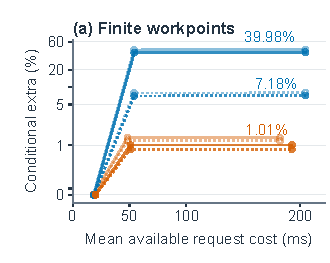
\includegraphics[width=.326\textwidth]{v4_figures/residual_results/opportunity_workpoints.pdf}\hfill
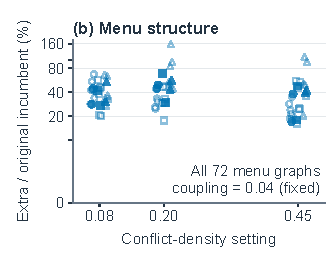
\includegraphics[width=.326\textwidth]{v4_figures/residual_results/opportunity_scenarios.pdf}\hfill
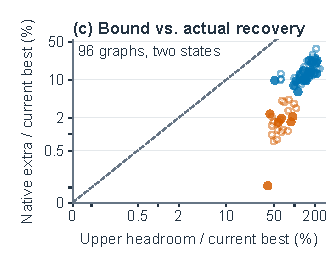
\includegraphics[width=.326\textwidth]{v4_figures/residual_results/opportunity_slack.pdf}

\includegraphics[width=.97\textwidth]{v4_figures/residual_results/opportunity_legend.pdf}
\caption{\textbf{Where additional joint recovery is available.}
Two actual snapshots per development graph.
(a) Best single-call admitted extra versus mean request cost; solid/dotted
curves normalize by original/current incumbents. (b) Menu topology and
density at fixed coupling 0.04. (c) Finite extra versus clique-bound headroom,
normalized by current best; diagonal: equality. Axes are linear near zero,
logarithmic beyond. These are conditional opportunities, not policy gains.}
\label{fig:conditional-recovery-opportunity}
\end{figure*}


\paragraph{Published whole-graph solver profiles.}
Table~\ref{tab:public-published-performance} retains all 17 published
configurations on 40 original public unit-weight graphs. Three runs are
averaged within each graph before equal-family aggregation. All 2,040
runs contribute, including 162 failed returns that preserve the initial
schedule. CHILS-p1 achieves 24.300\%/24.468\% accepted gain at the two
soft workpoints; the separate 16-thread configuration reaches
25.096\%/25.110\%. DIFUSCO's four-sample recipe improves accepted gain
over its one-sample recipe (12.313\% versus 8.724\%), with higher resident
request cost. COExpander's 6.347\% gain accompanies a 0.073\,s resident
cost. These observations characterize solver quality and cost on the
exposed inputs.

Native costs include startup, preprocessing, parsing and validation;
0.5/2\,s search allowances are not complete deadlines. Neural request
costs exclude the separately reported once-only setup. Released SAT-model
training overlap remains unresolved. No complete matched \method{} public
evaluation accompanies these profiles, so they do not establish its
transfer superiority or a speedup under matched total budgets.

\begin{table*}[t]
\centering
\caption{\textbf{Published whole-graph performance on 40 original public graphs.}
Three common initial schedules per graph; accepted gain is relative to the
original incumbent, with failures retaining its weight. Aggregation is
graph-first and family-balanced. Native cold costs and neural resident costs
have different boundaries.}
\label{tab:public-published-performance}
\footnotesize
\setlength{\tabcolsep}{5pt}
\begin{tabular}{@{}llrrrrrr@{}}
\toprule
& & \multicolumn{4}{c}{Accepted gain (\%) $\uparrow$} & & \\
\cmidrule(lr){3-6}
Method & Workpoint & DIMACS & UF & CBS & \textbf{Equal-family} & Cost (s) $\downarrow$ & Valid/120 $\uparrow$ \\
\midrule
\multicolumn{8}{@{}l}{\textbf{Native CPU: one thread; complete cold wall cost}} \\
CHILS-p1~\cite{grossmann2025chils} & 0.5\,s & 56.789 & 7.932 & 8.178 & 24.300 & 0.5455 & 120/120 \\
CHILS-p1~\cite{grossmann2025chils} & 2\,s & 57.235 & 7.961 & 8.209 & 24.468 & 2.0438 & 120/120 \\
$m^2$wis~\cite{grossmann2024mwis} & 0.5\,s & 25.428 & 7.383 & 7.833 & 13.548 & 4.1856 & 93/120 \\
$m^2$wis~\cite{grossmann2024mwis} & 2\,s & 25.428 & 7.383 & 7.833 & 13.548 & 5.5979 & 93/120 \\
$m^2$wis+s~\cite{grossmann2024mwis} & 0.5\,s & 25.428 & 7.162 & 7.491 & 13.360 & 4.1731 & 93/120 \\
$m^2$wis+s~\cite{grossmann2024mwis} & 2\,s & 25.428 & 6.967 & 7.566 & 13.320 & 5.5732 & 93/120 \\
Struction-fast~\cite{gellner2021struction} & 0.5\,s & 25.367 & 1.557 & 2.418 & 9.781 & 0.5519 & 120/120 \\
Struction-fast~\cite{gellner2021struction} & 2\,s & 36.260 & 1.915 & 2.645 & 13.607 & 2.0483 & 120/120 \\
Struction-strong~\cite{gellner2021struction} & 0.5\,s & 25.896 & 1.557 & 2.418 & 9.957 & 0.5482 & 120/120 \\
Struction-strong~\cite{gellner2021struction} & 2\,s & 36.177 & 1.924 & 2.645 & 13.582 & 2.0481 & 120/120 \\
WeightedBR (original)~\cite{lamm2019exact} & 0.5\,s & 13.376 & 4.975 & 6.147 & 8.166 & 3.8401 & 93/120 \\
WeightedBR (original)~\cite{lamm2019exact} & 2\,s & 13.902 & 6.723 & 7.686 & 9.437 & 5.2060 & 93/120 \\
\midrule
\multicolumn{8}{@{}l}{\textbf{Native CPU: 16 threads; complete cold wall cost}} \\
CHILS-p16-c16~\cite{grossmann2025chils} & 0.5\,s & 58.738 & 8.085 & 8.463 & 25.096 & 0.5505 & 120/120 \\
CHILS-p16-c16~\cite{grossmann2025chils} & 2\,s & 58.738 & 8.113 & 8.478 & 25.110 & 2.0494 & 120/120 \\
\midrule
\multicolumn{8}{@{}l}{\textbf{Released neural models: GPU; resident request cost}} \\
DIFUSCO-SAT~\cite{sun2023difusco} & $50\!\times\!1$ & 10.220 & 7.864 & 8.090 & 8.724 & 1.4209 & 120/120 \\
DIFUSCO-SAT~\cite{sun2023difusco} & $50\!\times\!4$ & 20.835 & 7.923 & 8.180 & 12.313 & 5.5737 & 120/120 \\
COExpander-SAT-CM~\cite{ma2025coexpander} & $1\!\times\!1$ & 7.553 & 5.644 & 5.844 & 6.347 & 0.0730 & 120/120 \\
\bottomrule
\end{tabular}
\par\smallskip
\begin{minipage}{\textwidth}
\footnotesize
Native workpoints are soft search allowances, not complete decision deadlines;
cold cost includes export, startup, preprocessing, parsing and validation.
Neural workpoints give steps $\times$ samples (DIFUSCO) or the released CM recipe
(COExpander). Once-only parent setup, excluded from resident cost:
DIFUSCO one/four samples: 5.948/5.946\,s; COExpander: 7.238\,s.
Costs are graph-first, equal-family means; valid counts retain all 120 runs.
\end{minipage}
\end{table*}


\section{Discussion and Limitations}
\label{sec:discussion-residual}

The results delimit the practical contribution. At the primary 0.556\,s
deadline, Capacity returns less improvement than the shared greedy policy;
the longer 2.221\,s budget permits additional recovery, but CheapSummary
achieves higher aggregate improvement than Capacity. These comparisons do
not establish an advantage for the structural learner. The contribution is
an execution-conditioned formulation and evaluation of coordinated recovery
beyond a common feasible response. Learned delegation and heuristic
scheduling already prioritize subsolver calls using execution
outcomes~\cite{li2021delegate,chmiela2021schedule}. Action-induced
compatibility, the warm anchor, and same-state supervision define the
specific prediction problem here. Graph message passing and clique bounds
remain established components whose inclusion provides no general
performance guarantee.

Conditional recovery opportunity and timely policy improvement differ.
All policies receive the same executed greedy prefix, so its improvement
cannot be attributed to learning. The complete caller deadline charges
preparation, prediction, executor calls, membership validation, and return.
A late result retains the original schedule under the stated metric, even
when a useful candidate existed internally. The high deadline-miss rate
therefore materially affects Capacity's primary result. Native soft search
allowances describe a different boundary. Point-value divided by expected
cost also omits runtime uncertainty and is a heuristic allocation rule;
valuable cloned responses alone cannot justify its effectiveness.

Post hoc diagnostics on a fixed training subset identify sensitivity to
request representation. Structural value summaries have much larger
magnitudes than the native-budget features, while predicted residual
fractions change little across workpoints whose executed extra values
differ. Most complete fitting histories have flat conditional allocation
regret, despite parameter updates and changing auxiliary losses. Some
scalar heads approach their warm floor; this does not support a conclusion
of network-wide gradient collapse. Unit imbalance is a plausible mechanism
for weak workpoint discrimination, but these observations neither isolate
the sole cause nor establish that normalization improves timed decisions.
Offline checkpoint regret evaluates one conditional choice and does not
optimize the complete multi-call return objective.

The bounds restrict scalar values; fractional occupancies need not be
integer schedules. Feasibility follows from checking actual memberships
against original conflicts. Ownership specifies participating agents without
establishing decentralized communication or privacy. Synthetic visibility
contacts omit orbital and operational uncertainty, and public ID partitions
are artificial. Published whole-graph solvers have different initialization
and scope contracts. Generalization beyond the observed domains and fixed
coupling remains unestablished. Failures and zero-opportunity graphs retain
their weight, fits are averaged within graphs, and the current development
results do not constitute independent confirmation.

\section{Conclusion}
Joint recovery links coordinated schedule improvement to finite feasible
solver responses. The proposed representation, bounded prediction and execution
supervision make that target explicit. Experiments distinguish conditional
opportunity from timely improvement: longer budgets permit additional recovery,
while inexpensive controls remain strong.

\clearpage
\balance
\bibliographystyle{ACM-Reference-Format}
\bibliography{references_v4_final}
\end{document}
